\chapter{Élément Technique}
%\addcontentsline{toc}{chapter}{Élément Technique}
\section{Parseur}
le parseur comme son nom l'indique constitue le cœur de notre application grâce à sa méthode 
génération permet de produire une chaîne  représentant un l-système végétal par réécriture en se servant d'un axiom de départ,un nombre d'itération  et des règles créée à partir de la classe \textbf{\em Rule} qu'il contient sous forme de liste .
\\
Pour qu'elle produise une chaîne représentant un l-système il faut se s'assurer que ses attributs aient été initialisés et qu'aucun d'entre eux  ne soit nul pour ceux de type entier et non vide pour ceux de type chaîne.En plus de ses attributs sa méthodes génération se sert également d'une méthode \textbf{\em compare} pour substituée chaque caractère par la chaîne devant le substituer suivant les règles définies.
\\
\\
l'algorithme de la génération d'un l-système par réécriture 
\\
	\begin{algorithm}
		\DontPrintSemicolon 
		\caption {Génération d'un l-système par réécriture  }
		\KwIn {axiom: $String$ , rules: $List[Rule]$ , nbIteration: $Integer$}
		\KwOut {Chaîne complète après la dernière itération}
		\For {$i \gets 0$ \textbf{à} $nbIteration$}{
				$production \leftarrow "" $ \;
				\For {$j \gets 0$ \textbf{à} $axiom.taille$}{
					$hasBeenUpdated \leftarrow faux $ \;
					\For {$Rule \ $r : $rules$}{
						\If{ $r.compare (axiom.charAt[j])$}{
							$hasBeenUpdated \leftarrow vrai $\;
							$production \leftarrow production + r.getItValues{} $ \;
							$arreter $\;
						}
					}
					\If{$!hasBeenUpdated $}{
							$production \leftarrow $production + $axiom.charAt[j] $ \;
					}
				}
				$axiom \leftarrow production $\;
		}
		\Return {$axiom$}\;
	\end{algorithm}
\section{Rule}
Elle permet de composer les règles d'un l-système  que la classe parser utilisera pour produire un system sous forme de chaîne avant que cette dernière ne soit interprétée  sous forme de rendu 2D ou 3D.Cette classe est très utile aussi car elle contient en son sein une méthode \textbf{\em compare} qui prends un caractère et retourne la chaîne devant le substituer lors d'une génération.


\section{Interface}
Nous avons utilisé l'interface java swing pour realiser l'interface utilisateur de notre application .Elle composée quatre (4) classes.
une permettant d'afficher la fenetre principale,une autre permettant de faire les Menu ,une troisième permettant defaire tout ce qui est configuration .

\subsection{FenetrePrincipale:}	
	Rassemble  tous les composants graphiques  menu,configuration et rendu. Elle constitue l'élément centrale gérant le lien entre le parseur et les modes de rendu.
\subsection{Configuration:}	\label{config}
	Définie les zones de paramétrage de l'application ainsi que les boutons de contrôle:
	\begin{itemize}
		 \item \textbf{Générate:} permettant générer un rendu 2D ou 3D du l-système;
		 \item \textbf{newRule:} pour ajouter au tant de règles souhaitées;
		 \item \textbf{clear:}  pour nettoyer les zone de textes et rendu .
	\end{itemize}
\subsection{Menu:}	
	Contient une liste déroulante de quelques exemples de l-systèmes sous format 2D et 3D, ainsi que l'option aide qui explique le fonctionnement du système. 
\subsection{Rendu:}
 Contient deux cases à cocher \textbf{rendu2d}, \textbf{rendu3d} permettant de choisir un mode de rendu ainsi qu'une zone de rendu pour la visualisation.
\section{Moteur graphique}
En ce qui concerne nos moteurs de rendu, nous utilisons du java swing pour le rendu 2D et jogl (java open gl library ) pour le rendu 3D .
	
\subsection{Rendu2D}
Nous utilisons du java swing pour faire le rendu 2D en redéfinissant la méthode \textbf{\textit{paintComponent(graphics 2d)}} de celui-ci. g2d.drawLine pour tracer les lignes(branche), g2d.translate pour faire des translations, g2d.scale pour gérer la mise en gras et une liste pour sauvegarder les positions si nécessaire.
\newpage
	\begin{figure}[h]
		 \centering
		 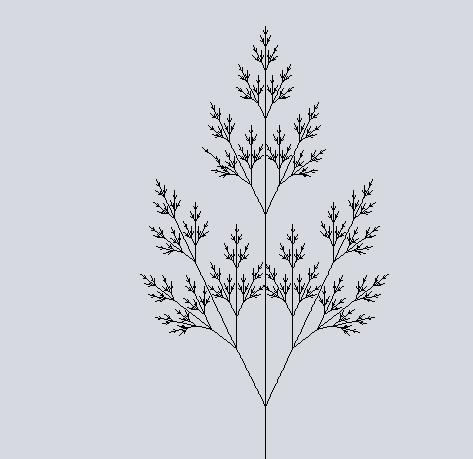
\includegraphics[width=7cm]{images/arbre2D.jpeg}
		 \caption{Exemple de rendu 2D}
		\end{figure}
	
\subsection{Rendu3D}
Comme mentionner ci-dessus, nous utilisons java openGL library pour faire notre rendu 3D notamment: gl2 pour afficher les lignes
glu pour placer la caméra et GLUT pour afficher les cylindres.
GLCanvas crée la fenêtre, GLEventListener initialise et affiche l’environnement 3D.
\\
	\begin{figure}[h]
		\centering
		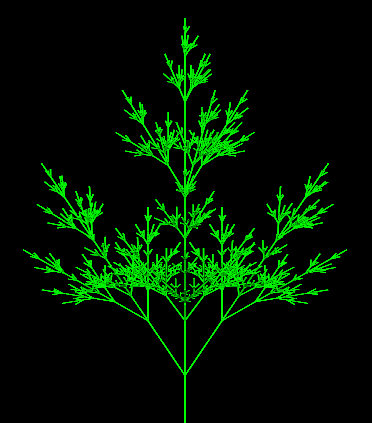
\includegraphics[width=7cm]{images/arbre3D.png}
	    \caption{Exemple de rendu 3D }
    \end{figure}
    	
